\chapter{Efficiencies}
\label{sec:Efficiencies}

The detection and reconstruction of particle decys is not perfect at all, i.e. not all particles and tracks happening in succession of a \proton\proton interaction are detected and recorded.
This discrepancy between the measured signal yields and the actually happened decays is summarized with the term ``efficiencies".
There are several reasons why different kinds of efficiencies occur.
Here are some examples:
\begin{itemize}
    \item Particles are flying out of the detector.
    \item A particle traverses a sensor in the deadtime, i.e. a signal caused by an earlier particle is still processed. 
          In this time, the sensor isn't able to process the second signal.
    \item Applying cuts for the reduction of background prevents signal events to pass these cuts as well
    \item ...
\end{itemize}
It's obvious that this list above is only the tip of the iceberg.
Nonetheless it's crucial to account for these efficiencies if one measures a physical quantity reliant on the number of events.
The way how the efficiencies for the \LbToDpmunuX and \LbToLcmunu enter the measurement of the relative branching ratio \R is shown in equation (\ref{eq:R}).

The determination of the efficiencies requires the use of simulations.
These simulation samples contain informations about all generated events as well as reconstructed events after the simulation of the detector. 
The naive way would be to divide the number of reconstructed MC events after applying all selection cuts and divide this by the number of generated events. 
This efficiency is hereafter called selection efficiency \effSel.
Nonetheless, the generation of the events isn't efficient at all. 
Several requirements are already applied during generation to reduce the computation time of the simulation production.
Above all the simulation of the detector takes a lot of time.
That's why all generated events are required to be in the \lhcb aceptance.
A further acceleration of the production process can be achieved with additional requirements on the final state particles' (transverse) momenta.
Concerning the  \LbToDpmunuX and \LbToLcmunu channel these requirements are different and likewise the efficiencies of the genration process.
Thus, the so called generator level efficiency \effGen also has to determined for both channels. 
The total efficiency used for the calculation of \R is then the product $\effGen \cdot \effSel$.

As life is not that easy the simulations don't perfectly describe the data. 
Above all the \LbToDpmunuX signal simulation doesn't contain a proper physics description and is thus in disagreement with data. 
Unfortunately, no theory prediction of the \LbToDpumnuX channel is available to fix this problem.
The plots in figure \ref{fig:reweighting} show a comparison of data (black points) and the simulation (red lines).
To get a better description of the decay the simulation hence has to be reweighted.
This should lead to a more proper estimate of the efficiency.
Several reweigthing steps are applied and will be described in the following.
\begin{figure}[hptb]
	\centering
	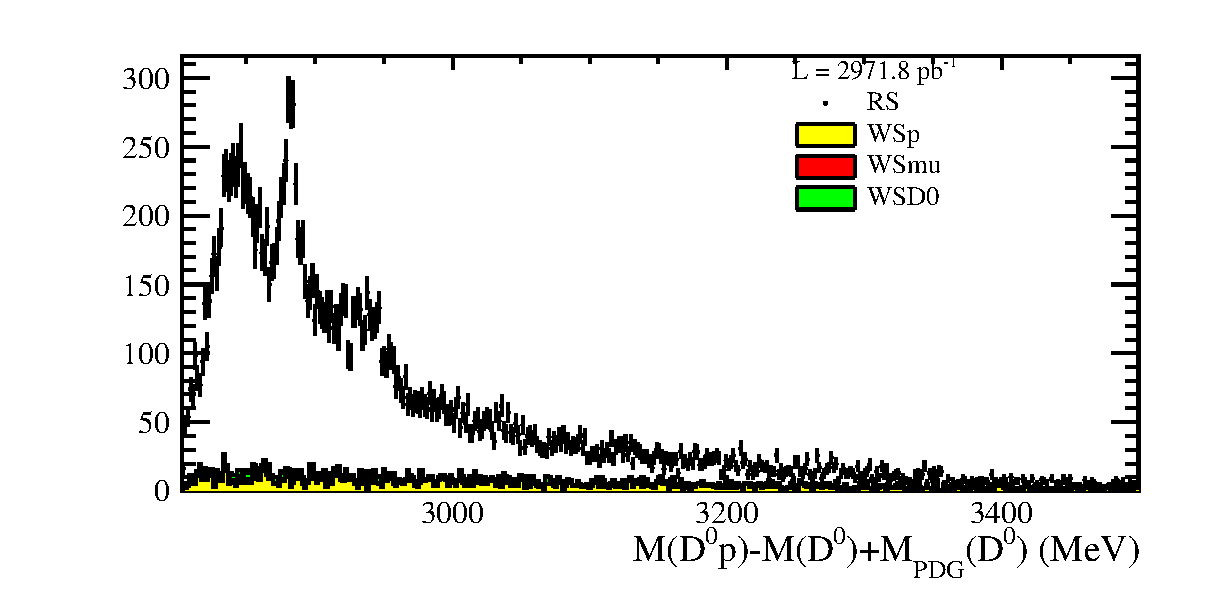
\includegraphics[width=0.49\textwidth]{LbToD0p/comparisons/3D/mD0p_mD0mu_mD0pmu/20Bins/20.0MaxWeight/Bh_DELTA_MASS}
	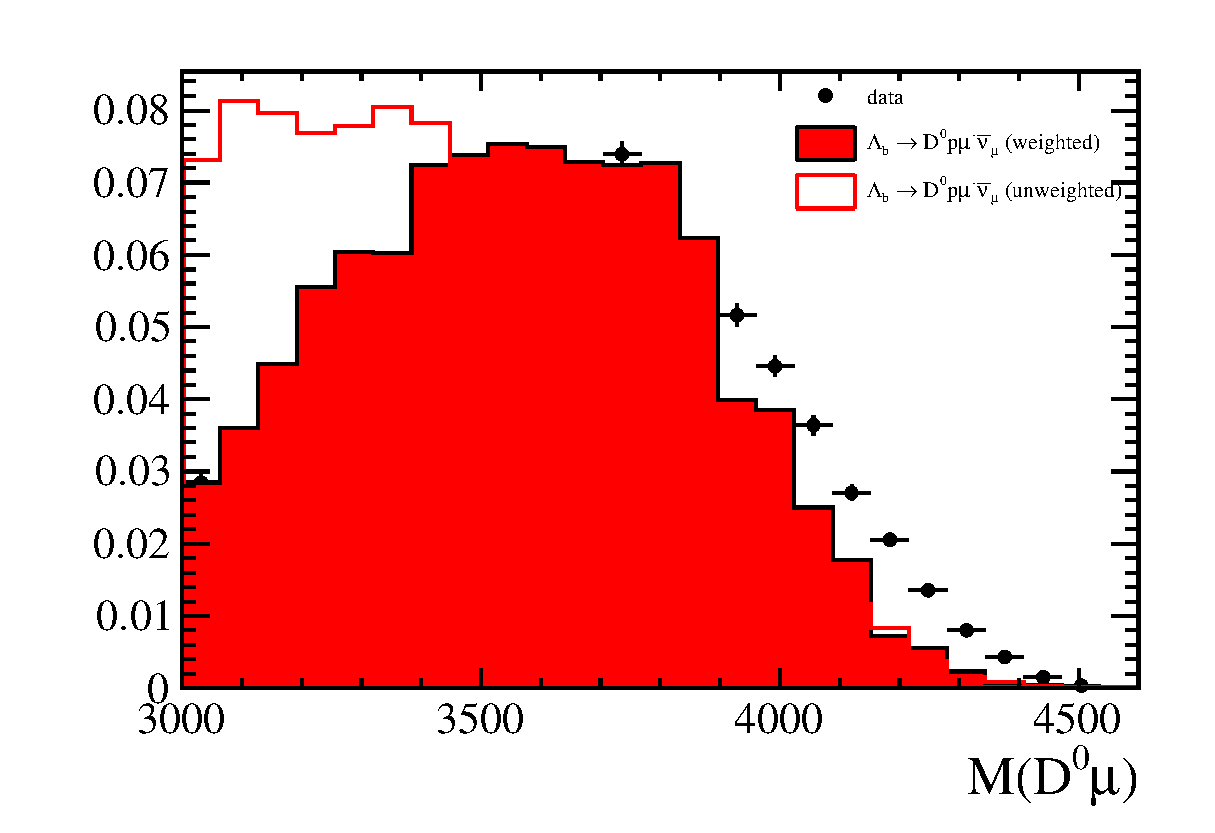
\includegraphics[width=0.49\textwidth]{LbToD0p/comparisons/3D/mD0p_mD0mu_mD0pmu/20Bins/20.0MaxWeight/B_M}
	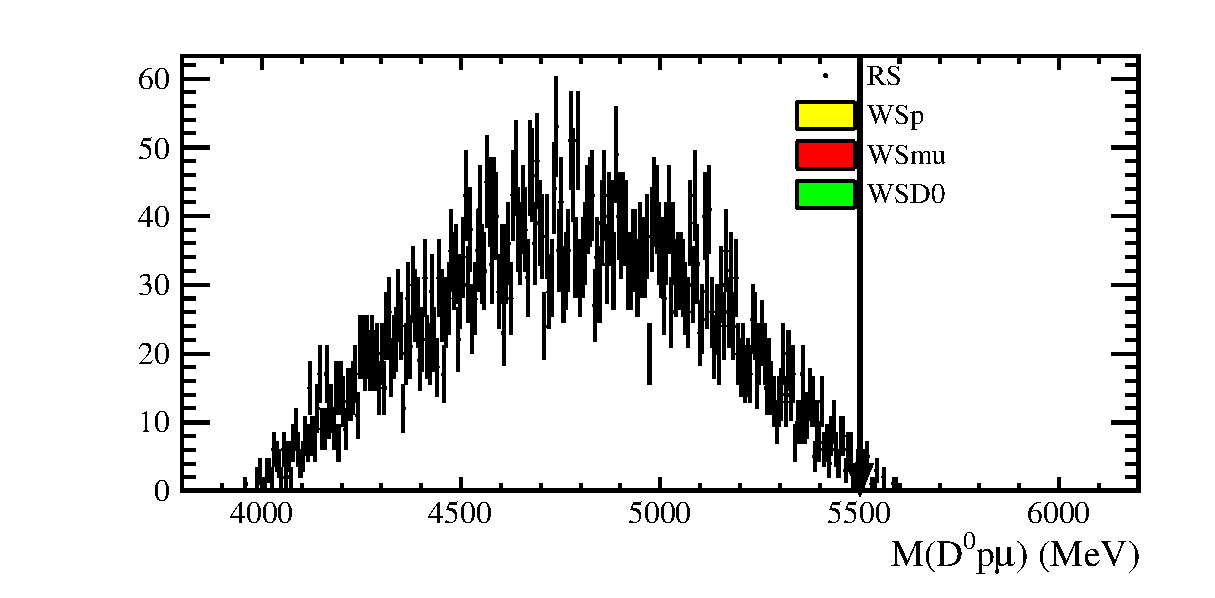
\includegraphics[width=0.49\textwidth]{LbToD0p/comparisons/3D/mD0p_mD0mu_mD0pmu/20Bins/20.0MaxWeight/Bh_M}
	\caption{Comparison of data (black points) and MonteCarlo prediction for the \LbToDpmunuX channel before (red line) and after (red shaded area) threedimensional reweighting as described in the text.}
	\label{fig:reweighting}
\end{figure}

\section{Kinematic reweighting of the \LbToDpmunuX and \LbToLcmunu channel}
The production of \Lb baryons depends strongly on their transverse momentum as figure \ref{fig:LbprodPT} from ref xxx shows. This dependence isn't well emulated by MC and has thus to be corrected. 
This was already done in ref xxx using the \decay{\Lb}{\jpsi\Dz\proton}. The weights they calculated are shown in figure \ref{fig:kinweights} and used to reweight both, \LbToDpmunuX and \LbToLcmunu channels, depending on their true \Lb transverse momentum \pt.

(\textbf{INCLUDE FIGURES FROM VUB ANALYSIS})


\section{Reweighting of the \Dz\proton signal MC}
\ref{sec:Reweight_D0p}

To reweight the \Dz\proton MC sample a threedimensional weighting in the variables
\begin{itemize}
    \item M(\Dz\proton)
    \item M(\Dz\mun)
    \item M(\Dz\proton\mun)
\end{itemize}
has been chosen. There are several reasons for this choice:
\begin{enumerate}
    \item their MC prediction is completely off from the data distribution,
    \item these variables are available as TRUE variables at generator and reconstruction level
    \item we don't cut at these variables\footnote{There exists a cut on M(\Dz\proton\mun) in this analysis to eliminate \decay{\Lb}{\Dz\proton\pim} background, but less than 0.5\% of all events have their TRUE mass above this cut. Thus, its impact on the efficiency can be neglected.}
\end{enumerate}
After the description of the reweighting and efficiency calculation process, it should become clear why these three points are important.
\begin{itemize}
    \item \textbf{Determination of the weights} \\
          There are two normalized 3D histograms drawn for both generated events (in the following called MCDecayTreeTuple or MCDTT) and events after reconstruction, applying selection cuts and the kinematic reweighting (DecayTreeTuple or DTT). 
          Both histograms have the three variables mentioned above on their axes.
          The histogram with the weights is now calculated by dividing the DTT histogram through the MCDTT histogram.
    \item \textbf{Assigning weights to the events} \\
          Now, this weight histogram is used to assign a weight to each DTT (\weight{DTT}) and MCDTT (\weight{MCDTT}) event.
          To get the correct bin in the weight histogram the true masses \Mtrue{\Dz\proton}, \Mtrue{\Dz\mun} and \Mtrue{\Dz\proton\mun} are used.
    \item \textbf{Calculation of the efficiency} \\
          The efficiency can now be calculated with
          \begin{align}
              \epsilon = \frac{\sum \weight{DTT}}{\sum \weight{MCDTT}}, \label{eq:effrew}.
          \end{align}
          To account for the loss of statistical power due to weighting, both numerator and denominator in equation \ref{eq:effrew} are multiplied by the renormalisation factor $\sum \weight{MCDTT} / \sum \weight{DTT}^2$. 
          This doesn't affect the central value of $\epsilon$ but influences the statistical error, which is calculated using binomial statistics.
\end{itemize}
It should now be clear, that we must not cut on the weighting variables, since otherwise we shouldn't now which weight has to be assigned to the MCDTT. The distribution of the masses after reweighting are also shown in figure \ref{fig:reweighting}.

\section{Generator level efficiencies}
The MC generation for the \LbToDpmunuX and \LbToLcmunu has different efficiencies. The so called ``decProdCut" requires the generated particles to be in the \lhcb acceptance during MC production. 
For example, in the case of our normalization mode \LbToLcmunu this means the \Lc and the \muon point towards \lhcb.

For signal and normalization channel we obtain the following generator level efficiencies:
\begin{align*}
    \effGenLc &= \effGenLcval \pm \effGenLcerr, \\
    \effGenDp &= \effGenDpval \pm \effGenDperr.
\end{align*}

\section{Reconstruction and selection efficiencies}
The reconstruction and selection efficiencies are calculated as described above. Whereas the \Dz\proton channel is reweighted twice (kinematic \pt(\Lb) and 3D mass reweighting) there's only the kinematic reweighting applied for the \Lc channel. The results are:
\begin{align*}
    \effSelLc &= \num[scientific-notation=true]{\effSelLcval \pm \effSelLcerr}, \\
    \effSelDp &= \num[scientific-notation=true]{\effSelDpval \pm \effSelDperr}.
\end{align*}

\section{Total efficiencies}
To summarise the values above the total efficiencies for the channels are:
\begin{align*}
    \effDp &= \effGenDp \cdot \effSelDp = \num[scientific-notation=true]{\effDpval \pm \effDperr}, \\
    \effLc &= \effGenLc \cdot \effSelLc = \num[scientific-notation=true]{\effLcval \pm \effLcerr}.
\end{align*}
For the consideration of systematics later it is sometimes more useful to consider the ratio of both efficiencies
\begin{align*}
    \frac{\effLc}{\effDp} = \effRatioval \pm \effRatioerr.
\end{align*}
